\documentclass{lehramt-informatik-aufgabe}
\liLadePakete{uml}
\begin{document}
\liAufgabenTitel{Firmenstruktur}
\section{1 Firmenstruktur
\index{Einfach-verkettete Liste}
\footcite{examen:46116:2011:03}}

\begin{center}
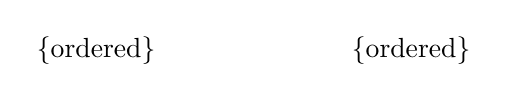
\begin{tikzpicture}
\node (ordered1) at (2,3) {\{ordered\}};
\node (ordered2) at (6,3) {\{ordered\}};

\umlclass[x=0]{Firma}{}{+ addAbteilung(name: String)\\+ erzeugelDs()}
\umlclass[x=4.5]{Abteilung}{+ name: String}{}
\umlclass[x=8]{Angestellter}{+ id: int}{}
\umlassoc[arg1=+ firma,mult1=1,pos1=0.7]{ordered1}{Firma}
\umlassoc[arg1=+ abteilungen,mult1=*,pos1=0.5]{ordered1}{Abteilung}
\umlassoc[arg1=+ abteilung,mult1=1,pos1=0.7]{ordered2}{Abteilung}
\umlassoc[arg1=+ angestellte,mult1=*,pos1=0.7]{ordered2}{Angestellter}
\end{tikzpicture}
\end{center}

\noindent
Eine Firma besteht aus null oder mehr Abteilungen, von denen jede null
oder mehr Angestellte hat. Da sowohl die Abteilungen als auch deren
Angestellten geordnet sind, sind Angestellte insgesamt geordnet. Sie
haben durchgehende, ganzzahlige IDs, die bei 1 beginnen.

\begin{enumerate}

%%
% a)
%%

\item Erstellen Sie exemplarisch ein Objektdiagramm: Stellen Sie eine
Firma mit dem Instanznamen f und den zwei Abteilungen „Produktion“ (Name
p) und „Marketing“ (Name m) dar. Die Produktion hat zwei Angestellte,
Marketing hat einen Angestellten. Die Angestellten haben die Namen a1,
a2, und a3.

\begin{liAntwort}
Die Instanzbezeichnung müsste noch unterstrichen werden. Das geht aber
leider mit TikZ-UML nicht.
\begin{center}
\begin{tikzpicture}

\umlclass[x=0,y=0]{f : Firma}{}{}

\umlclass[x=0,y=-2]{p : Abteilung}{name = “Produktion”}{}
\umlclass[x=4,y=-2]{m : Abteilung}{name = “Marketing”}{}

\umlclass[x=0,y=-4,name=a1]{a1 : Angestellter}{id = “1”}{}
\umlclass[x=3,y=-4]{a2 : Angestellter}{id = “2”}{}
\umlclass[x=6,y=-4]{a3 : Angestellter}{id = “3”}{}

\umluniassoc{f : Firma}{p : Abteilung}
\umluniassoc{p : Abteilung}{m : Abteilung}
\umluniassoc{p : Abteilung}{a1 : Angestellter}
\umluniassoc{a1 : Angestellter}{a2 : Angestellter}

\umluniassoc{m : Abteilung}{a3 : Angestellter}

\end{tikzpicture}
\end{center}
\end{liAntwort}

%%
% b)
%%

\item Implementieren Sie das Klassendiagramm in Java oder in einer
anderen geeigneten objektorientierten Programmiersprache Ihrer Wahl.
Beachten Sie, dass die Assoziationen bidirektional und geordnet sind.
Die beiden Methoden der Klasse Firma sollen dabei folgendes Verhalten
haben:

- Die Methode erzeugelDs sorgt dafür, dass die IDs wieder korrekt
zugewiesen sind. Die alten IDs können beliebig geändert werden, solange
das Endergebnis wieder den obenstehenden Kriterien genügt.

%%
% c)
%%

\item Angestellte sollen in Manager und einfache Angestellte unterteilt
werden. Zeichnen Sie ein Klassendiagramm mit der Oberklasse
Angestellterund den zwei Unterklassen Manager und EinfacherAngestellter.
Die Klasse Angestellter soll nicht instantiierbar sein und erzwingen,
dass die Methode getPosition() (öffentlich, ohne Argumente, Rückgabewert
String) von allen konkreten Unterklassen implementiert wird. Manager und
EinfacherAngestellter sollen instantiierbar sein.

%%
% d)
%%

\item Wie lautet der Fachbegriff dafür, dass eine Methode in einer
Klasse und in deren Unterklassen dieselbe Signatur hat, aber in den
Unterklassen unterschiedlich implementiert ist?

\end{enumerate}

\end{document}
